\documentclass[../main]{subfiles}
\begin{document}

\chapter{模型的建立}%
\label{cha:establishment}

\section{数据预处理}%
\label{sec:preprocess}

\subsection{采集}%
\label{sub:gather}

收集到的数据经过初步整理和汇总后,可以分为基础数据表~\ref{tab:basic}、日数据
表~\ref{tab:day}和年数据表~\ref{tab:year}。以2011年作为第一年,以此类推。

\begin{table}[htbp]
  \centering
  \caption{基础数据}%
  \label{tab:basic}
  \csvautobooktabular{tab/basic.csv}
\end{table}

\begin{table}[htbp]
  \centering
  \caption{日数据}%
  \label{tab:day}
  \tiny
  \csvautobooktabular{tab/day.csv}
\end{table}

\begin{table}[htbp]
  \centering
  \caption{年数据}%
  \label{tab:year}
  \tiny
  \setlength\tabcolsep{2pt}
  \csvautobooktabular{tab/year.csv}
\end{table}

通过股票编号和年份就可以将对应的年数据和日数据整合到一张数据表内,由此便可以
将原本分散在日数据表年数据表中的因子数据整合到一起进行分析。对于基本数据表中
的数据,我们利用编码将每个行业映射为一组数字,由于股票为次新股对是否实施高送
转的影响大\cite{邢小艳基于模式识别的“高送转”投资策略研究,
王悦上市公司高送转的影响因素分析},我们只从基本数据表中提取出次新股、所属行业
属性并按相同的方法将其整合入数据表,以这个数据表作为我们的数据集。

\subsection{插值}%
\label{sub:value_lose_process}

建立模型所使用的原始数据中存在着数据的缺失,因此必须对缺失值进行一定的处理已
减小其对模型的影响。

如果一个因子的数据缺失过多,就放弃使用这个因子,对于存在较多数据缺失的因子,
我们将其滤去,因为缺失太多数据的因子数据难以确定其对实施高送转的影响。

如果缺失值较少,就利用数据之间存在的关系采用拉格朗日插值法来表示缺失值$y(x)$
:从原始数据中取出缺失值前后的共$k$个数据$y(x_j), j = 0, 2, \ldots, k - 1$,
用根据定义~\ref{def:lagrage}得到的$L_k(x)$表示$y(x)$。

\begin{definition}[拉格朗日插值法]%
  \label{def:lagrage}
  根据式~\ref{eq:lagrage}得到的$L_k(x)$。
\end{definition}

\begin{align}
  \label{eq:lagrage}
  L_k(x) = & \sum_{j = 0}^{k - 1} y(x_j) \ell_j(x)\\
  \ell_j(x) = & \prod_{i\in \mathbb{Z}_n - \{i\}}\frac{x-x_i}{x_j-x_i}
\end{align}

\subsection{标准化}%
\label{sub:standard}

不同因子数据之间可能存在较大的数量级的差距。若将差距较大的数据一起进行建模时
,他们之间的差距会对模型产生很大的影响。为了消除不同因子数据之间量纲的不同,
我们对数据进行标准化。在模型构建的过程中。我们将会使用两种将数据标准化的方法
并进行准确性的比对。

\begin{definition}[0--1标准化]
  通过式~\ref{eq:01}将$x$转换到$[0, 1]$之间的值$x'$。
\end{definition}

\begin{definition}[均值方差标准化]
  通过式~\ref{eq:ed}将$x$转换到均值为0 ,方差为1的值$x''$。
\end{definition}

\begin{align}
  \label{eq:01}
  x' = & \frac{x-\min{X}}{\max{X} - \min{X}}\\
  \label{eq:ed}
  x'' = & \frac{x - \bar{x}}{\sigma}\\
  \bar{x} = & \frac{1}{\lvert X\rvert}\sum_{x \in X} x\\
  \sigma = & \sqrt{\frac{1}{\lvert X\rvert}\sum_{x \in X}{(x - \bar{x})}^2}
\end{align}

\section{主成分分析}%
\label{sec:factor}

\subsection{因子的选取}%
\label{sub:factor_chosen}

挑选出对高送转股票具有较大影响的因子越多,往往都可以提升因子模型的准确性,但
选择过多的因子又会导致模型的计算量成几何增长。而过少的因子又可能无法完全覆盖
股票的完全信息。因此所选取的因子应当具有鲁棒性、可解释性、可持续性的特征。

高积累、高股价和股本小是上市公司实施高送转的先决条件,次新股、股本扩张与业绩
一致增长的股票也具有较强的高送转意愿。同时,政策的变化以及时间的滞后效应也会
影响到上市公司是否实施高送转的决策。因此从总体上来看,影响上市公司是否实施高
送转会受到基本因子、成长因子、时序因子和政策因子的影响。

根据上述原因,我们选出了部分因子构建成因子池如表~\ref{tab:pca}的第一列所示。

主成分分析可以将原来的多个变量重新组合成一组新的相互无关的几个综合变量,同时
根据实际需要从中可以取出几个较少的总和变量尽可能多地反映原来变量的信息的统计
。通过主成分分析,我们可以得到载荷矩阵$P$如表~\ref{tab:pca}。当所选取的主成分
$F_1, F_2, \ldots, F_n$的贡献率达到85\%以上时,那么对应的主成分就能够反应原有
的变量信息了。

\begin{table}[htpb]
  \centering
  \caption{因子变量的载荷矩阵}%
  \label{tab:pca}
  \scriptsize
  \csvautobooktabular{tab/pca.csv}
\end{table}

由上述结果,我们选取了十四个对上市公司实施高送转方案有较大影响的因子,其因子
名称和因子定义如表~\ref{tab:factor}所示。我们将得到的因子设定为自变量,上市公
司是否实施高送转作为0--1因变量。

\begin{table}[htpb]
  \centering
  \caption{选取的因子变量}%
  \label{tab:factor}
  \scriptsize
  \csvautobooktabular{tab/factor.csv}
\end{table}

\subsection{特征选择}%
\label{sub:character_select}

首先我们基于决策树进行特征选择,得到各因子对因变量的重要性和各变量的相关系数
分别如表~\ref{tab:importance}、表~\ref{tab:correlation_current}所示。

我们将所有的数据按比例划分为训练数据和测试数据。

\begin{table}[htpb]
  \centering
  \caption{因子对高送转变量的重要性}%
  \label{tab:importance}
  \csvautobooktabular{tab/importance.csv}
\end{table}

\begin{table}[htpb]
  \centering
  \caption{各因子的相关系数}%
  \label{tab:correlation_current}
  \tiny
  \setlength\tabcolsep{2pt}
  \csvautobooktabular{tab/correlation_current.csv}
\end{table}

从表~\ref{tab:importance}中可以发现,每个变量对高转送变量的重要性相差不大,但
根据表~\ref{tab:correlation_current}中我们发现,每股净资产和每股资本公积、每
股未分配利润的相关性很大,均达到了0.75以上,因此我们剔除每股净资产这一因子以
减少变量的个数。

将部分相关性太大的因子剔除后,新的因子之间的相关系数如
表~\ref{tab:correlation}所示。

\begin{table}[htpb]
  \centering
  \caption{剔除部分因子后的相关系数}%
  \label{tab:correlation}
  \tiny
  \setlength\tabcolsep{2pt}
  \csvautobooktabular{tab/correlation.csv}
\end{table}

递归特征消除的主要思想是反复的构建模型的特征,把选出来的特征放到一遍,然后在
剩余的特征上重复这个过程,直到所有特征都遍历了。这个过程中特征被消除的次序就
是特征的排序。这是一种寻找最优特征子集的算法。

通过进行特征递归消除以及进行交叉验证,我们得到了图~\ref{fig:REF_choose}。

\begin{figure}[htbp]
  \centering
  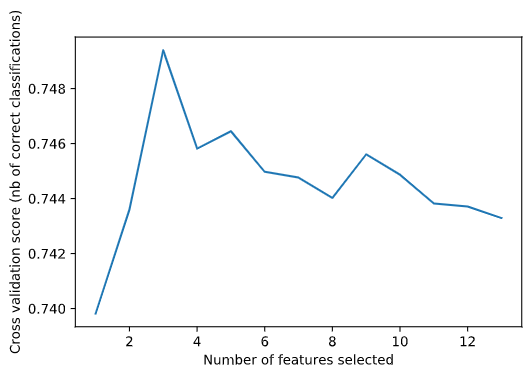
\includegraphics[
    width = 0.8\linewidth,
  ]{fig/REF_choose}
  \caption{RFE以及交叉验证}%
  \label{fig:REF_choose}
\end{figure}

REF可以衡量随着特征数目的增加,模型分类准确率的变化情况,通过这一原理我们可以
来确定最优的特征数目。随着自变量数目的增加,模型的交叉检验准确率一直在上升。
因此我们保留这几个因子变量作为我们预测是否实施高送转的自变量。

\subsection{分类}%
\label{sub:classify}

在进行模型构建和预测之前应当对数据集进行分类,我们将数据集分为训练集和测试集
。划分的思路为:假设现在是第$n$年,那么我们将第$n - 1, n - 2$年的数据作为训练
集,第$n$年的数据作为测试集。我们的评估方法为:将测试集代入使用训练集训练过的
模型中,将测试集按照股票实施高送转的概率排序,选取其中概率最大的10、25、50、
100支股票,并同时通过实际数据计算出这些股票在现实中实施高送转的概率
。\cite{胡宸2019基于集成学习的上市公司高送转预测模型及投资策略设计,
  江鹏基于支持向量机(SVM)股票择时策略的研究,
  凤河有限注意与A股市场股价回归预测--基于SVM与Logistic的比较研究
}

在进行模型构建和预测之前应当对数据集进行分类,我们将数据集分为训练集和测试集
。划分的思路为:假设现在是第$n$年,那么我们将第$n - 1, n - 2$年的数据作为训练
集,第$n$年的数据作为测试集。我们的评估方法为:将测试集代入使用训练集训练过的
模型中,将测试集按照股票实施高送转的概率排序,选取其中概率最大的10、25、50、
100支股票,并同时通过实际数据计算出这些股票在现实中实施高送转的概率。

将两种不同的标准化方法和不采用标准化三种数据处理方法作为横坐标,将概率最大的
10、20、50、100支股票作为纵坐标。我们注意到数据集中的正负样本数量不均匀,如果
不加以处理可能会导致超平面被\enquote{推向}负类,也即不实施高送转,影响结果的
准确性。因此我们对两个类别的样本进行均衡,这样在模型训练过程中每个类别的特征
都会在一定程度上被学习。

\section{时间序列分析}%
\label{sec:analyse}

\subsection{Logistic回归模型}%
\label{sub:logistic}

Logistic回归是一种广义的线性回归,可用式~\ref{eq:logistic}表述。其中$\bm{x}$
是输入,可以是连续型变量也可以为离散型变量。$\bm{\theta}$为待求参数。因变量$y
= 0$表示结果不发生,$y = 1$表示结果发生。

\begin{align}
  \label{eq:logistic}
  P\{y = 1\mid \bm{x};\bm{\theta}\} = & h_{\bm{\theta}}(\bm{x}) =
  \frac{1}{1 + \exp{(-\bm{\theta}^\mathsf{T}\bm{x})}}\\
  P\{y = 0\mid \bm{x};\bm{\theta}\} = & 1 - P\{y = 1\mid \bm{x};\bm{\theta}\}
\end{align}

根据式~\ref{eq:c}设置的代价函数$C(\tilde{y}_{\bm{\theta}})$能够衡量模型的好坏
,其中$\tilde{y}_{\bm{\theta}}$是根据式~\ref{eq:y}得到的对$y$的估计误差。根据
式~\ref{eq:j}设置目标函数$J(\bm{\theta})$。训练模型的过程也就是不断地改变
$\bm{\theta}$,从而得到更小的目标函数$J(\bm{\theta})$的过程。

\begin{align}
  \label{eq:c}
  C(\tilde{y}_{\bm{\theta}}) = & -\ln\lvert \tilde{y}_{\bm{\theta}}\rvert\\
  \label{eq:y}
  \tilde{y} = & h_{\bm{\theta}}(\bm{x}) - y\\
  \label{eq:j}
  J(\bm{\theta}) = & \mathop{\mathrm{E}}_{\bm{x}}C(\tilde{y}_{\bm{\theta}})
\end{align}

梯度下降中的梯度指的是代价函数对各个参数的偏导数,偏导数的方向决定了在学习过
程中参数下降的方向,学习率$\alpha$决定了每步变化的步长,有了导数和学习率就可
以使用梯度下降算法的公式~\ref{eq:theta}来求解使$J(\bm{\theta})$最小的参数
$\bm{\theta}$。

\begin{align}
  \label{eq:theta}
  \tilde{\theta}_j = \theta_j -
  \alpha\pdv{\theta_j}J(\bm{\theta}) = \theta_j -
  \frac{\alpha}{m}\sum^{m}_{i = 1}(h_{\bm{\theta}}(\bm{x}^{(i)}) -
  y^{(i)})x_j^{(i)}
\end{align}

过滤掉今年前三季度以及进行高送转的股票,我们可以得到基于Logistic模型的不同选
股个数、不同标准化方法下的预测准确度如表~\ref{tab:logistic}所示。

\begin{table}[htpb]
  \centering
  \caption{第3--7年基于Logistic模型的预测}%
  \label{tab:logistic}
  \setlength\tabcolsep{2pt}
  \begin{subtable}[htbp]{0.45\linewidth}
    \centering
    \caption{第3年基于Logistic模型的预测}%
    \label{tab:logistic3}
    \csvautobooktabular{tab/logistic3.csv}
  \end{subtable}
  \qquad
  \begin{subtable}[htbp]{0.45\linewidth}
    \centering
    \caption{第4年基于Logistic模型的预测}%
    \label{tab:logistic4}
    \csvautobooktabular{tab/logistic4.csv}
  \end{subtable}

  \begin{subtable}[htbp]{0.45\linewidth}
    \centering
    \caption{第5年基于Logistic模型的预测}%
    \label{tab:logistic5}
    \csvautobooktabular{tab/logistic5.csv}
  \end{subtable}
  \qquad
  \begin{subtable}[htbp]{0.45\linewidth}
    \centering
    \caption{第6年基于Logistic模型的预测}%
    \label{tab:logistic6}
    \csvautobooktabular{tab/logistic6.csv}
  \end{subtable}

  \begin{subtable}[htbp]{0.45\linewidth}
    \centering
    \caption{第7年基于Logistic模型的预测}%
    \label{tab:logistic7}
    \csvautobooktabular{tab/logistic7.csv}
  \end{subtable}
\end{table}

可以看出,Logistic模型预测的准确性与所使用的标准化方式并无太大的关系,并且其
预测的准确性随着年份的增长逐渐增加,并且对少数股票的预测结果准确性高。

\subsection{支持向量机SVM模型}%
\label{sub:svm}

支持向量机是在分类与回归分析中分析数据的监督式学习模型与相关的学习算法。除了
进行线性分类之外,SVM还可以使用核技巧有效的进行非线性分类。
根据式~\ref{eq:T}给定一个特征空间上的训练数据集$T$

\begin{align}
  \label{eq:T}
  T = \{(\bm{x}^1, y^1), (\bm{x}^2, y^2), \ldots, (\bm{x}^N, y^N)\}
\end{align}

其中$\bm{x}^i \in \mathbb{R}^n, y^i \in \{1, -1\}, i = 1, 2, \ldots, N$。我们
的目标是找到一个超平面$\bm{\omega}\cdot\bm{x} + b = 0$,使其关于所有样本点的
几何间隔的取到最小值$\gamma = \min\limits_{i = 1, 2, \ldots, N}\gamma^i$,
$\gamma^i$表示几何间隔。

那么SVM模型的求解最大分割超平面问题可以表示为约束最优化问题的公式~\ref{eq:b}
。

\begin{align}
  \label{eq:b}
  \min_{\bm{\omega}, b}
  \frac{1}{2}\lVert\bm{\omega}\rVert^2\qquad\mathrm{s.t.}
  y^i(\bm{\omega}\cdot\bm{x}^i + b)\geqslant 1, i = 1, 2, \dots, N
\end{align}

通过与Logistic模型相类似的方法,我们可以得到基于SVM模型的准确度如
表~\ref{tab:svm}所示。

\begin{table}[htpb]
  \centering
  \caption{第3--7年基于SVM模型的预测}%
  \label{tab:svm}
  \setlength\tabcolsep{2pt}
  \begin{subtable}[htbp]{0.45\linewidth}
    \centering
    \caption{第3年基于SVM模型的预测}%
    \label{tab:svm3}
    \csvautobooktabular{tab/svm3.csv}
  \end{subtable}
  \qquad
  \begin{subtable}[htbp]{0.45\linewidth}
    \centering
    \caption{第4年基于SVM模型的预测}%
    \label{tab:svm4}
    \csvautobooktabular{tab/svm4.csv}
  \end{subtable}

  \begin{subtable}[htbp]{0.45\linewidth}
    \centering
    \caption{第5年基于SVM模型的预测}%
    \label{tab:svm5}
    \csvautobooktabular{tab/svm5.csv}
  \end{subtable}
  \qquad
  \begin{subtable}[htbp]{0.45\linewidth}
    \centering
    \caption{第6年基于SVM模型的预测}%
    \label{tab:svm6}
    \csvautobooktabular{tab/svm6.csv}
  \end{subtable}

  \begin{subtable}[htbp]{0.45\linewidth}
    \centering
    \caption{第7年基于SVM模型的预测}%
    \label{tab:svm7}
    \csvautobooktabular{tab/svm7.csv}
  \end{subtable}
\end{table}

从表格中我们可以看出,SVM模型得到的预测结果波动性较大,而且标准化方式不同,其
预测的准确性也存在较大的区别,并且对于少数股票的预测准确性存在较大的误差,稳
定性不够好。与Logistic模型得到的结果进行对比,SVM预测得到的准确性与Logistic预
测得到的准确性只有部分年份相差较大,并且在第六年预测的准确度明显低于其余的年
份。

\subsection{基于逻辑回归与支持向量机的高送转预测模型}%
\label{sub:logistic_svm}

使用SVM模型进行预测的结果在不同年份时其准确性变化较大,Logistic模型和SVM模型
单独使用都存在着或多或少的缺陷,因此我们将两个模型结合起来。同时使用两种模型
进行预测,我们的评估方法也进行了相应的调整,具体的步骤为:

\begin{enumerate}
  \item 分别使用Logistic模型和SVM模型进行实施高送转的预测,按照概率大小进行排
    序,基于排序基于所得到的排序进行打分。
  \item 将两个模型的得分相加,按照总得分的顺序进行排序。
\end{enumerate}

我们得到了不同年份的模型准确性表格如表~\ref{tab:logistic_svm}所示。

\begin{table}[htpb]
  \centering
  \caption{第3--7年基于Logistic和SVM模型的预测}%
  \label{tab:logistic_svm}
  \setlength\tabcolsep{2pt}
  \begin{subtable}[htbp]{0.45\linewidth}
    \centering
    \caption{第3年基于Logistic和SVM模型的预测}%
    \label{tab:logistic_svm3}
    \csvautobooktabular{tab/logistic_svm3.csv}
  \end{subtable}
  \qquad
  \begin{subtable}[htbp]{0.45\linewidth}
    \centering
    \caption{第4年基于Logistic和SVM模型的预测}%
    \label{tab:logistic_svm4}
    \csvautobooktabular{tab/logistic_svm4.csv}
  \end{subtable}

  \begin{subtable}[htbp]{0.45\linewidth}
    \centering
    \caption{第5年基于Logistic和SVM模型的预测}%
    \label{tab:logistic_svm5}
    \csvautobooktabular{tab/logistic_svm5.csv}
  \end{subtable}
  \qquad
  \begin{subtable}[htbp]{0.45\linewidth}
    \centering
    \caption{第6年基于Logistic和SVM模型的预测}%
    \label{tab:logistic_svm6}
    \csvautobooktabular{tab/logistic_svm6.csv}
  \end{subtable}

  \begin{subtable}[htbp]{0.45\linewidth}
    \centering
    \caption{第7年基于Logistic和SVM模型的预测}%
    \label{tab:logistic_svm7}
    \csvautobooktabular{tab/logistic_svm7.csv}
  \end{subtable}
\end{table}

第三年到第七年不同预测模型的准确性折线图如图~\ref{fig:Acuuracy}所示。

\begin{figure}[htbp]
  \centering
  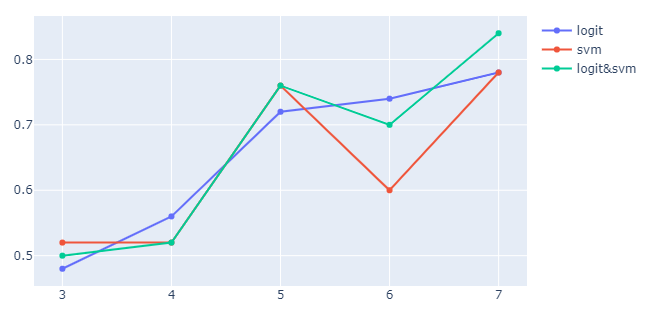
\includegraphics[
    width = 0.8\linewidth,
  ]{fig/Accuracy}
  \caption{不同预测模型的准确性}%
  \label{fig:Acuuracy}
\end{figure}

通过分析表格~\ref{tab:logistic_svm}和图~\ref{fig:Acuuracy},我们可以得出:将
两个模型结合使用后,相对于单独使用两种模型,预测的准确性变得更加稳定,同时不
同标准化方式对预测结果的影响也较小。并且我们可以看到对50支股票进行预测的准确
性达到了80\%,因此我们在对第八年股票进行预测的时候该模型预测的结果是比较可靠
的。

\end{document}

